\section{Experiments}
\label{sec:experiments}
Porting the models to the new framework is only the first part of this thesis. Once the models have been ported, I have only shown that the framework is flexible enough to embody these models. However, without being able to reproduce the same results, it would be like shoving the triangular piece down the square slot. It will fit eventually, but completely defeats the purpose. It is important that for the framework to be viable, it should be able to show that the outcome has not changed. The model should produce the same results regardless of the fact that it has been ported to a new platform. As you might've guessed, this chapter is about reproducing past results. A few experiments will be re-conducted and the results represented and compared to the old results. We will also be looking at the small improvements made to ArtDev3D, and see how they perform compared to the original implementation.


\subsection{Developing 3D shapes using ArtDev3D's model}
For this model, the sphere and the x-mas tree was chosen to test the new implementation of ArtDev3D. The reason for choosing these two, is because the sphere is a relatively simple shape to evolve and easily achieve perfect fitness. It will be perfect for testing the accuracy of the re-implementation. The reason the normal tree is not chosen is because it is very similar to the x-mas tree in shape, and it is almost as complex. On top of that, ArtDev3D does equally well on both of these. The purpose of the second test is to see how well the new implementation will do on difficult shapes.

Both of these experiments were conducted with different settings in H{\o}ye's paper\cite{hoye2006} in order to see how various parameters would affect the fitness of the individuals. In this thesis, however, a fixed set of parameters was used for simplicity's sake. The numbers may therefore deviate from the original results because this decision. However, the experiments were run with settings as close to the original experiments as possible:

\begin{itemize}
	\itemsep=-2pt
	\item Population: 1 000
	\item Generations: 500
	\item Mating rate: 90\%
	\item Mutation rate: 10\%
	\item Crossover: Single point
	\item Selection: Tournament (size=4, pressure=0.8)
\end{itemize}

\noindent And the parameters used for development:

\begin{itemize}
	\itemsep=-2pt
	\item Development time: 12 ticks
	\item Protein lifespan: 5 ticks
	\item Cell types: 1 (sphere) / 12 (x-mas tree)
	\item Chemical types: 1
	\item Don't-care-neighbours: 6
\end{itemize}

The experiments were run 200 times. H{\o}ye reported to have run these experiments 980 times each but with varying parameters. Considering there are many set-ups he could have run them with, a smaller number was chosen now because only one set-up is used. 200 runs should be enough to demonstrate the point of this chapter.

\subsubsection{Sphere}
\begin{center}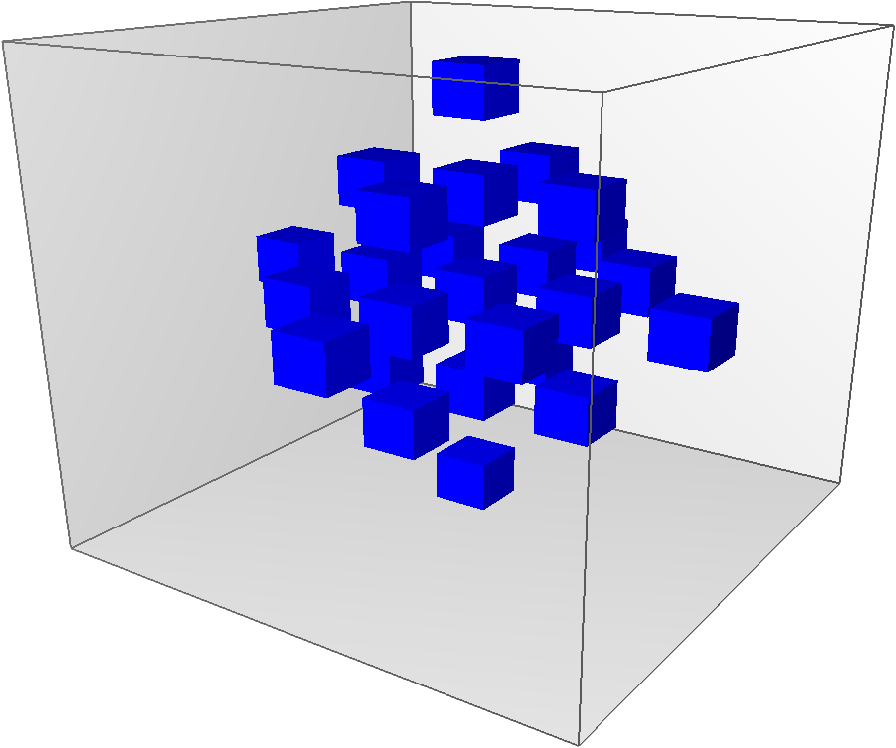
\includegraphics[scale=0.2]{sphere}\end{center}
This shape seems the simplest to evolve as it is entirely symmetrical and much less complex than other shapes. Since these experiments are about verifying that everything runs as it should, they will always use the same parameters. The number of perfect specimens found was recorded and presented in figure~\ref{fig:chart_artdev3d_sphere}.

\begin{figure}[!ht]
	\centering
	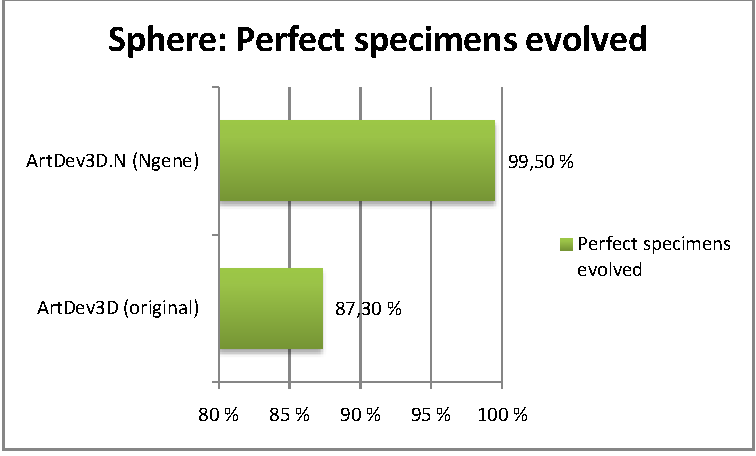
\includegraphics[scale=0.9]{chart_artdev3d_sphere}
	\caption{ArtDev3D: Sphere results}
	\label{fig:chart_artdev3d_sphere}
\end{figure}

Original ArtDev3D managed to evolve perfect fitness in 856 out of 980 experiments. It is important to remember that these were run with \emph{different} settings whereas we are using the best settings available here. That is why we see a much higher percentage (199 out of 200) than the original experiments. Had we known what these parameters were beforehand and used them, the number would probably have been much closer to the original results. Regardless, it does show that the development framework can perform equally well.

\subsubsection{X-mas tree}
\begin{center}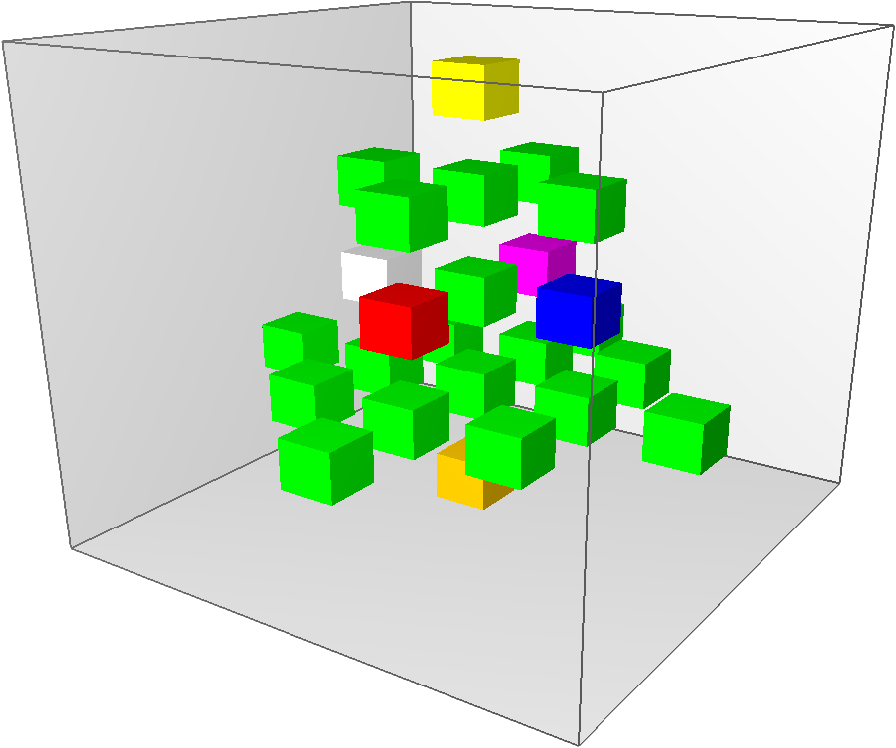
\includegraphics[scale=0.2]{x-mas-tree}\end{center}
This experiment is of a different nature than the previous one. It may not be very scientific but should demonstrate how well Ngene performs on complex shapes compared to ArtDev3D. No perfect specimens are expected here because ArtDev3D had a hard time evolving one, and it is not expected for Ngene to outperform it. The highest fitness after each run was recorded for figure~\label{fig:chart_artdev3d_x-mas-tree}.

\begin{figure}[!ht]
	\centering
	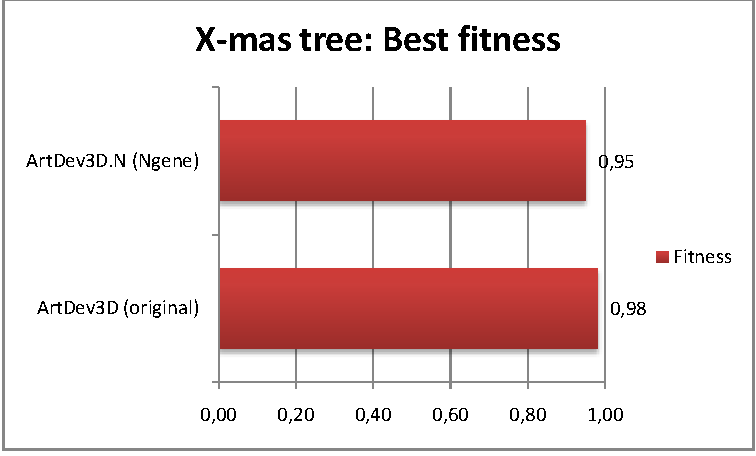
\includegraphics[scale=0.9]{chart_artdev3d_x-mas-tree}
	\caption{ArtDev3D: X-mas tree results}
	\label{fig:chart_artdev3d_x-mas-tree}
\end{figure}

It seems that Ngene is performing rather well. Note that the highest fitness achieved in ArtDev3D only occurred once in the 980 test runs. This experiment is but a fifth of that, and it is not inconceivable that Ngene might be able to achieve higher fitness with a larger sample. Interestingly, Ngene only managed to evolve fitness above 0.9 in 57 out of 200 runs. The rest were above 0.8 however. This tells us how well the model copes with complex shapes.

\subsubsection{Summary}
We've seen that the new implementation of ArtDev3D can evolve on an equal level as the original implementation. In chapter~\ref{sec:Implementation:ArtDev3D}, I've mentioned that there was a fix applied to the model when it was ported to the framework. From what can be seen above, it would seem that this patch has not affected the model in any perceivable way. Whether or not the fix is beneficial in any way, is difficult to see. It may very well be that the bug is dormant.


\subsection{Developing the French flag using artificial development}
For the re-implementation of ADCGP model, the French flag experiment was picked out. The purpose of this experiment is to evolve a grid of cells that resembles the French flag. Each cell is given a type of either blue, red or white. For every cell that corresponds with the target, one point is rewarded. The fitness is calculated from the total points scored divided by maximum score achievable. The engine ran with the following settings:

\begin{itemize}
	\itemsep=-2pt
	\item Population: 100
	\item Generations: 10 000
	\item Mating rate: 90\%
	\item Mutation rate: 30\%
	\item Crossover: Single point
	\item Selection: Tournament (size=4, pressure=0.8)
\end{itemize}

\noindent The target phenotype used:

\begin{center}\fbox{
\includegraphics{French-flag}}\end{center}

Finding the right development time for this particular problem proved to be rather difficult. It would seem that setting the development time too high not only slowed down the whole process, it also made it harder for the organisms to evolve correctly. The experiments started out with development time of 10 ticks and was slowly decremented as the results were not satisfactory. The following are the best evolved organisms using 4 ticks.

\begin{center}
	\fbox{
\includegraphics{cartesian-4-3-90-9-3-20081119-083309}}
	~\fbox{
\includegraphics{cartesian-4-3-90-9-3-20081119-091139}}
	~\fbox{
\includegraphics{cartesian-4-3-90-9-3-20081119-230852}}
\end{center}

It seemed odd that setting the development time one step longer would have any saying in how the organisms would grow. To ensure that the results weren't purely coincidental, the experiment was repeated once more for five ticks.

\begin{center}
	\fbox{
\includegraphics{cartesian-5-3-90-9-3-20081120-221123}}
	~\fbox{
\includegraphics{cartesian-5-3-90-9-3-20081120-233001}}
	~\fbox{
\includegraphics{cartesian-5-3-90-9-3-20081121-002613}}
\end{center}

These results seem to suggest that the model is not stable. Colours appear in areas they shouldn't be in as opposed to the previous results where the colours at least stayed closer to each other. Note that there is a hole in the middle flag, next to the red cell in the blue area. One can theorize that the growth continues even after target phenotype has been evolved, hence resulting in a worse fitness. This seems to be backed up by the fact that the engine would more frequently obtain fitness above 0.9 when using development time of four when compared to five. Using development time of 10 also raised the number of cells above 200.

To further investigate this issue, the phenotype was altered so that it would have a border around the flag.

\begin{center}\fbox{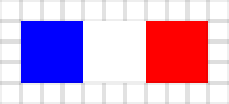
\includegraphics{French-flag-border}}\end{center}

\noindent This new phenotype will hopefully show whether or not the model does continue to grow, or if it manages to maintain a status quo to some extent. No changes were made to the settings above. The tests were repeated using the new target phenotype.

\begin{center}
	Development time: 4 ticks\newline
	\fbox{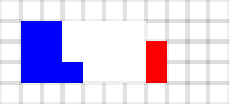
\includegraphics{cartesian-4-3-90-9-3-20081120-071044}}
	~\fbox{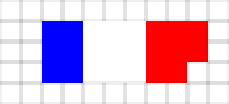
\includegraphics{cartesian-4-3-90-9-3-20081120-081439}}
\end{center}

\begin{center}
	Development time: 5 ticks\newline
	\fbox{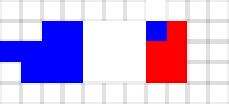
\includegraphics{cartesian-5-3-90-9-3-20081121-063215}}
	~\fbox{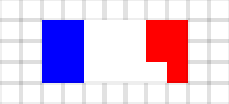
\includegraphics{cartesian-5-3-90-9-3-20081121-072947}}
	~\fbox{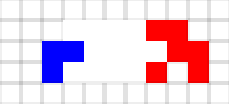
\includegraphics{cartesian-5-3-90-9-3-20081121-205507}}
\end{center}

As suspected, the average fitness dropped due to the increased size and complexity of the phenotype. With the exception of the first flag in the second row that ``bleeds'' into the border (two cells: blue on the left and white cell above the one blue cell in red cells zone), all of them are missing cells for some reason. It seems like the model compensates by either growing less cells or initiating cell death more often. Unfortunately, the results can't be called conclusive due to the nature of test. One will have to look into how the organisms change in each development step. The tools necessary for this is unavailable at the moment.

Another interesting thing to note is that the bug mentioned in section~\ref{sec:cartesian} had little to no effect on any of the results above. In fact, the no-bug version seem to achieve higher fitness more frequently than the bugged version by a small margin. This conflicts with what Dr. Miller reported.


\subsection{Performance Benchmarks}
With regards to what has been written about ArtDev3D up to this point, I've only discussed the potential performance gain of this framework without showing anything concrete. We shall now put these claims under scrutiny, and see how fast the new ArtDev3D, cleverly dubbed ArtDev3D\emph{.N} (N for Ngene or N-hanced), really is. This simple benchmark test was run on an Intel\textregistered Core\texttrademark 2 Duo E6300 with 2 GB of DDR2-RAM under Linux 2.6.27-7. The conditions of the programs under run:

\begin{itemize}
	\itemsep=0pt
	\item ArtDev3D ran with Java\texttrademark SE Runtime Environment 6 Update 10 build 33.
	\item ArtDev3D.N was compiled with GCC 4.3.2, with optimization flags: \texttt{-O3}.
	\item Additionally, ArtDev3D.N was also compiled with Intel\textregistered C++ Compiler (ICC) 11.0 build 069, with optimization flags: \texttt{-xHost -fast}.
\end{itemize}

\noindent The same settings were used for both engines:

\begin{itemize}
	\itemsep=-2pt
	\item Population: 100
	\item Generations: 100
	\item Mating rate: 90\%
	\item Mutation rate: 30\%
	\item Development time: 12 ticks
	\item Target: Sphere
\end{itemize}

\noindent Perfect termination was disabled so that the engines would not exit when perfect fitness was found. This is to ensure that both engines ran for the exact same number of generations. The test was repeated 100 times and the average time was then calculated.

\begin{figure}[!ht]
	\centering
	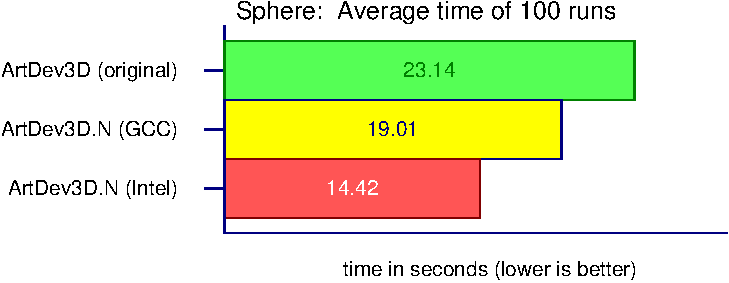
\includegraphics[scale=0.9]{chart_avg-time}
	\caption{ArtDev3D vs. ArtDev3D.N: Speed}
	\label{fig:chart_avg-time}
\end{figure}

The speed gained (fig.~\ref{fig:chart_avg-time}) here is quite significant considering that the sample is relatively small to perform a benchmark on. Using an open source compiler such as GCC, Ngene is faster than ArtDev3D by 4.13 seconds. This is to be expected as C++ is faster than Java. We also see that switching to a better compiler like ICC shaved off an additional 4.59 seconds, making the gap 8.72 seconds. The optimizations flags were not experimented with so the gap could potentially be increased even more. The framework itself can still be optimized further as well. We will have a discussion regarding this topic in chapter~\ref{sec:improvements}. Speed aside, it is also interesting to see how they perform memory-wise. These numbers were taken during the experiments above.

\begin{figure}[!ht]
	\centering
	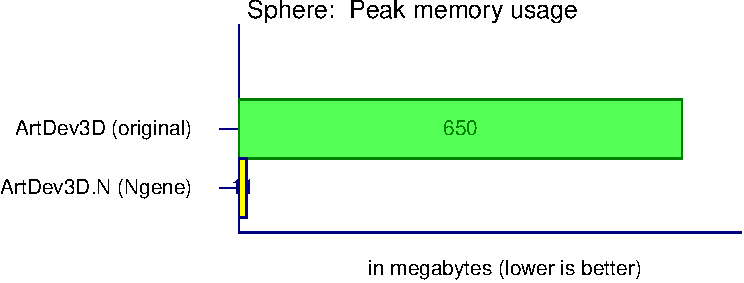
\includegraphics[scale=0.9]{chart_peak-memory-usage}
	\caption{ArtDev3D vs. ArtDev3D.N: Memory usage}
	\label{chart_peak-memory-usage}
\end{figure}

Figure~\ref{chart_peak-memory-usage} shows that ArtDev3D peaks at a staggering 650 MB! The average is only a few MB less. The main culprit for this is Java\texttrademark Virtual Machine. It has been criticized\cite{maio2008} for the garbage collector because of its ridiculous memory consumption. The reason behind is that during allocation and de-allocation, it leaves the memory very fragmented and has a hard time filling the gaps in between, resulting in more memory allocated without being used entirely. Memory usage is important because lowering memory use can also increase overall performance. The computer that these experiments were conducted on has 2 MB of L2 cache. If a program fit into this cache, it would run significantly faster than a program that doesn't. Ngene peaks out at 11 MB but averages at around 7 MB during a run.
